\section{Robotic Data Acquisition System Setup}
\begin{frame}
	\frametitle{Robotic Data Acquisition System Setup}
	\begin{figure}[hbt!]
		\centering
		\begin{subfigure}{0.4\textwidth}
			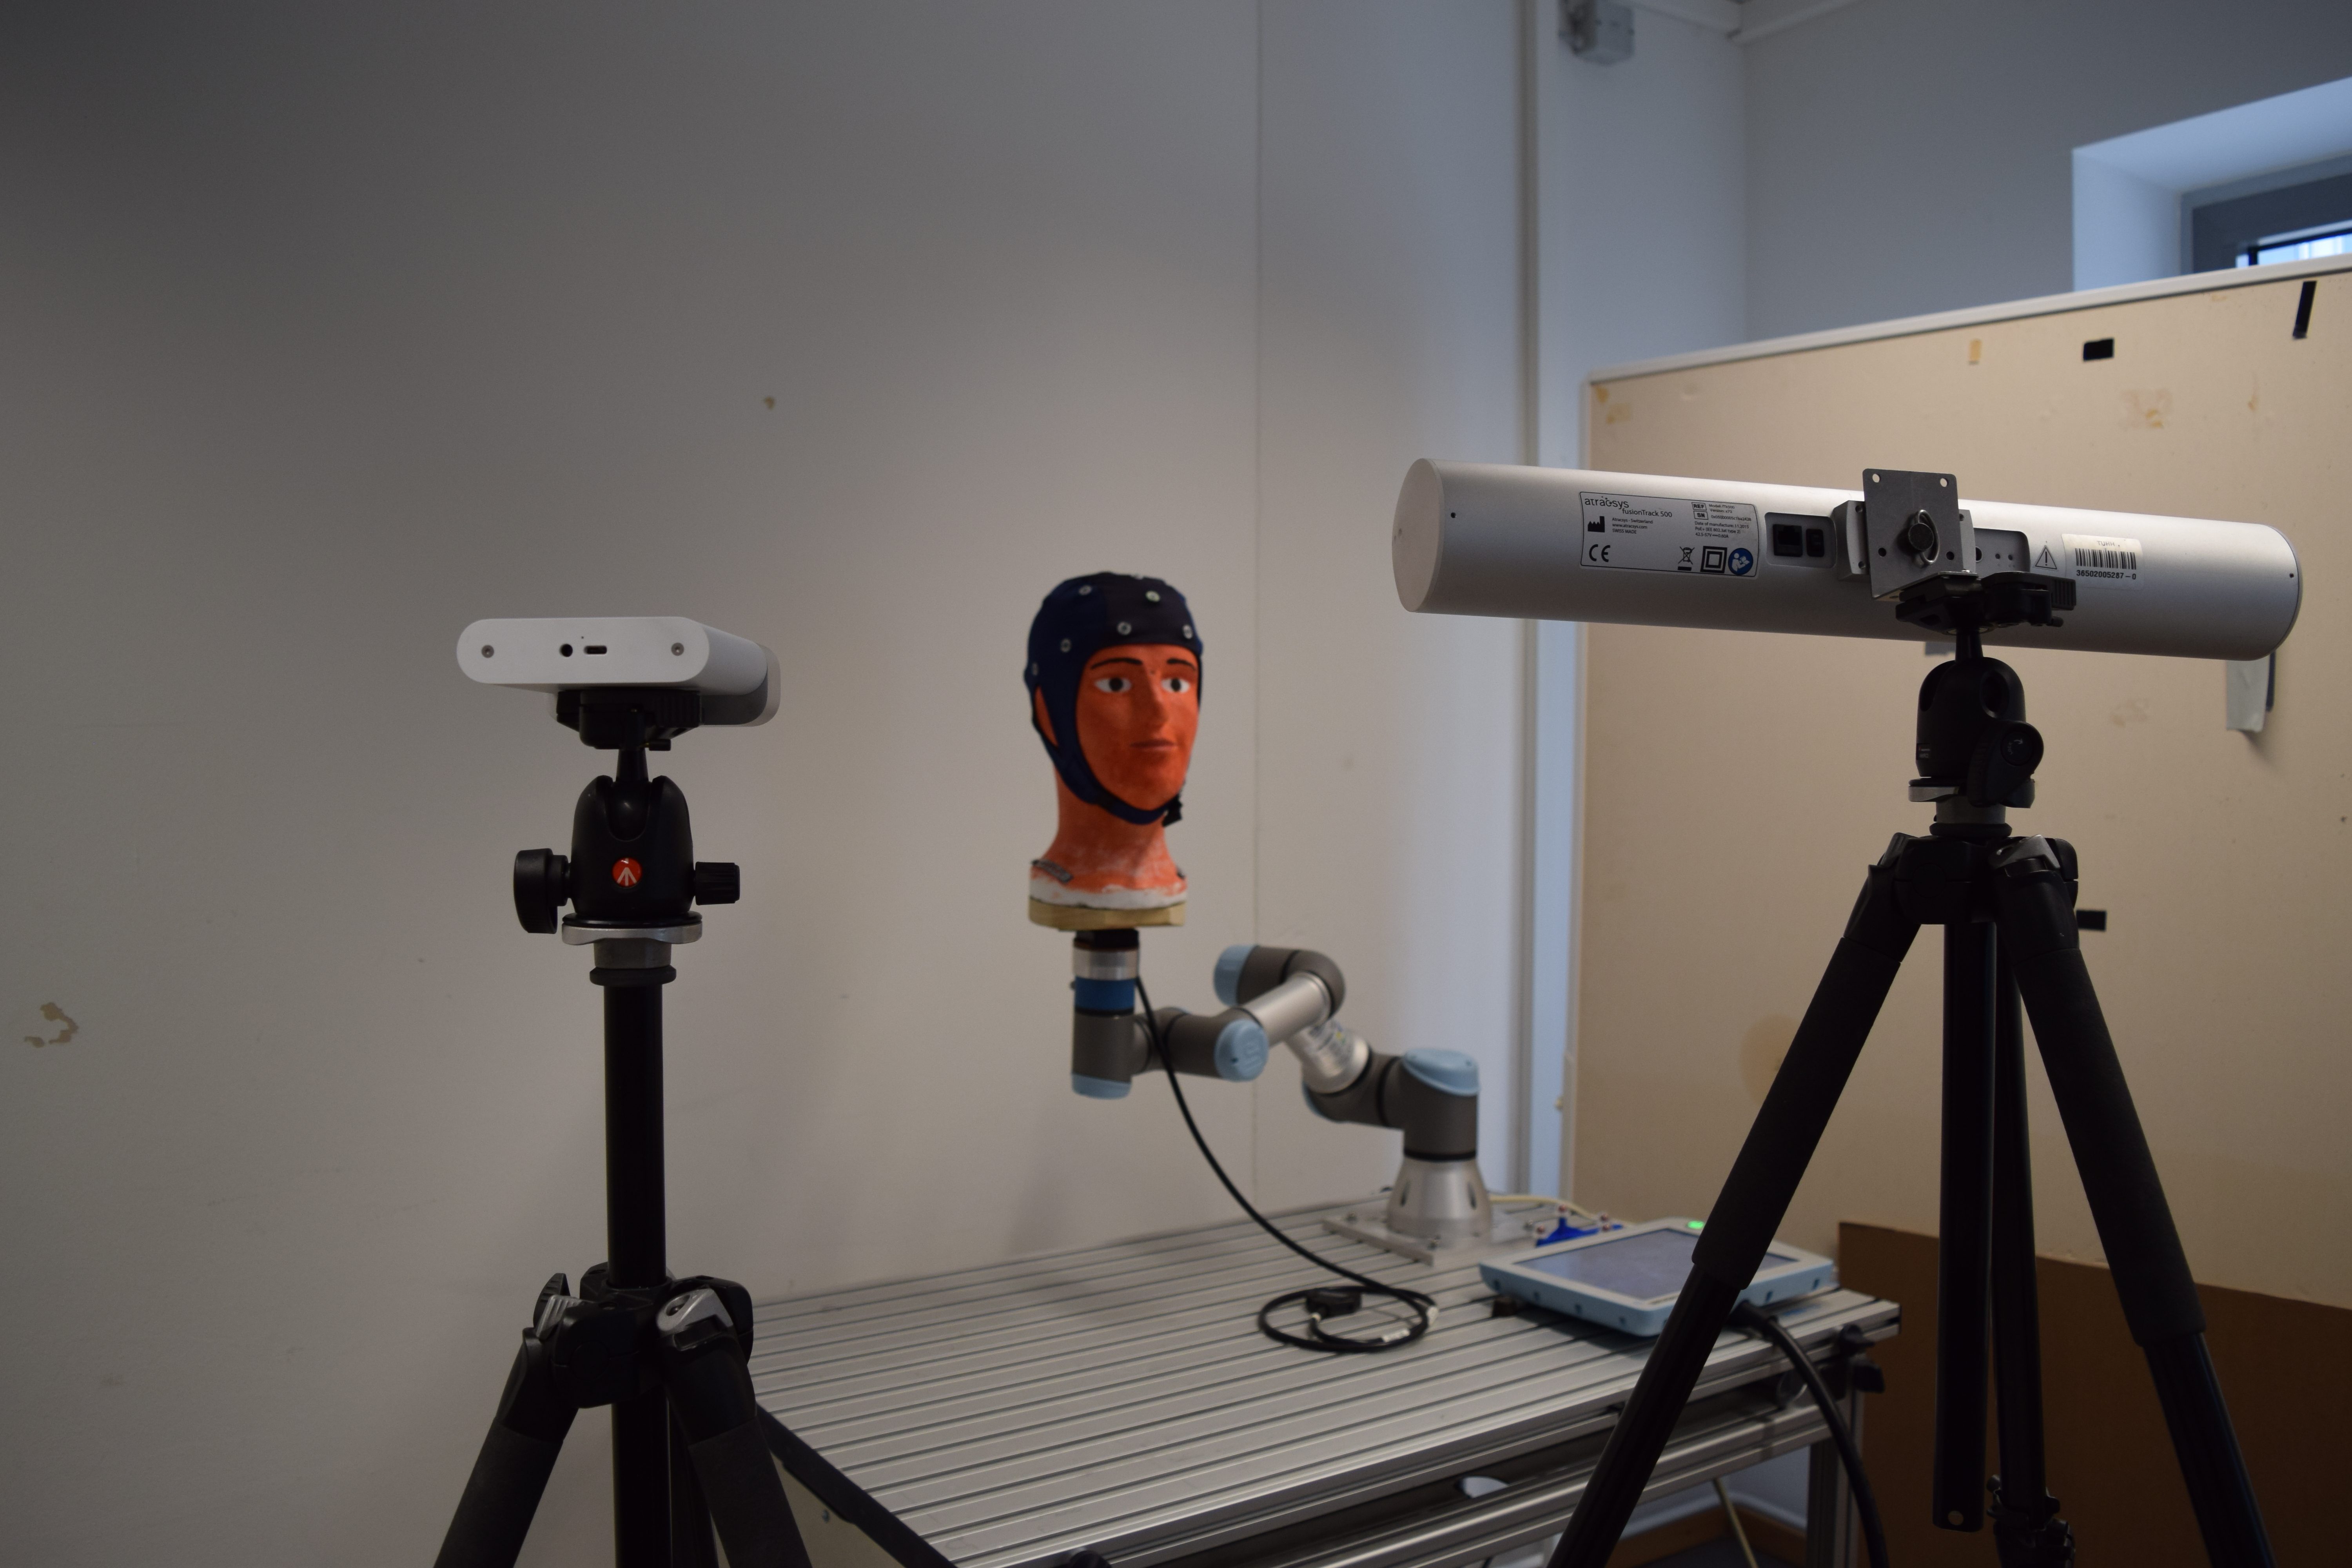
\includegraphics[width=\textwidth]{experimental_setup_1.jpg}	
		\end{subfigure}
		\begin{subfigure}{0.4\textwidth}
			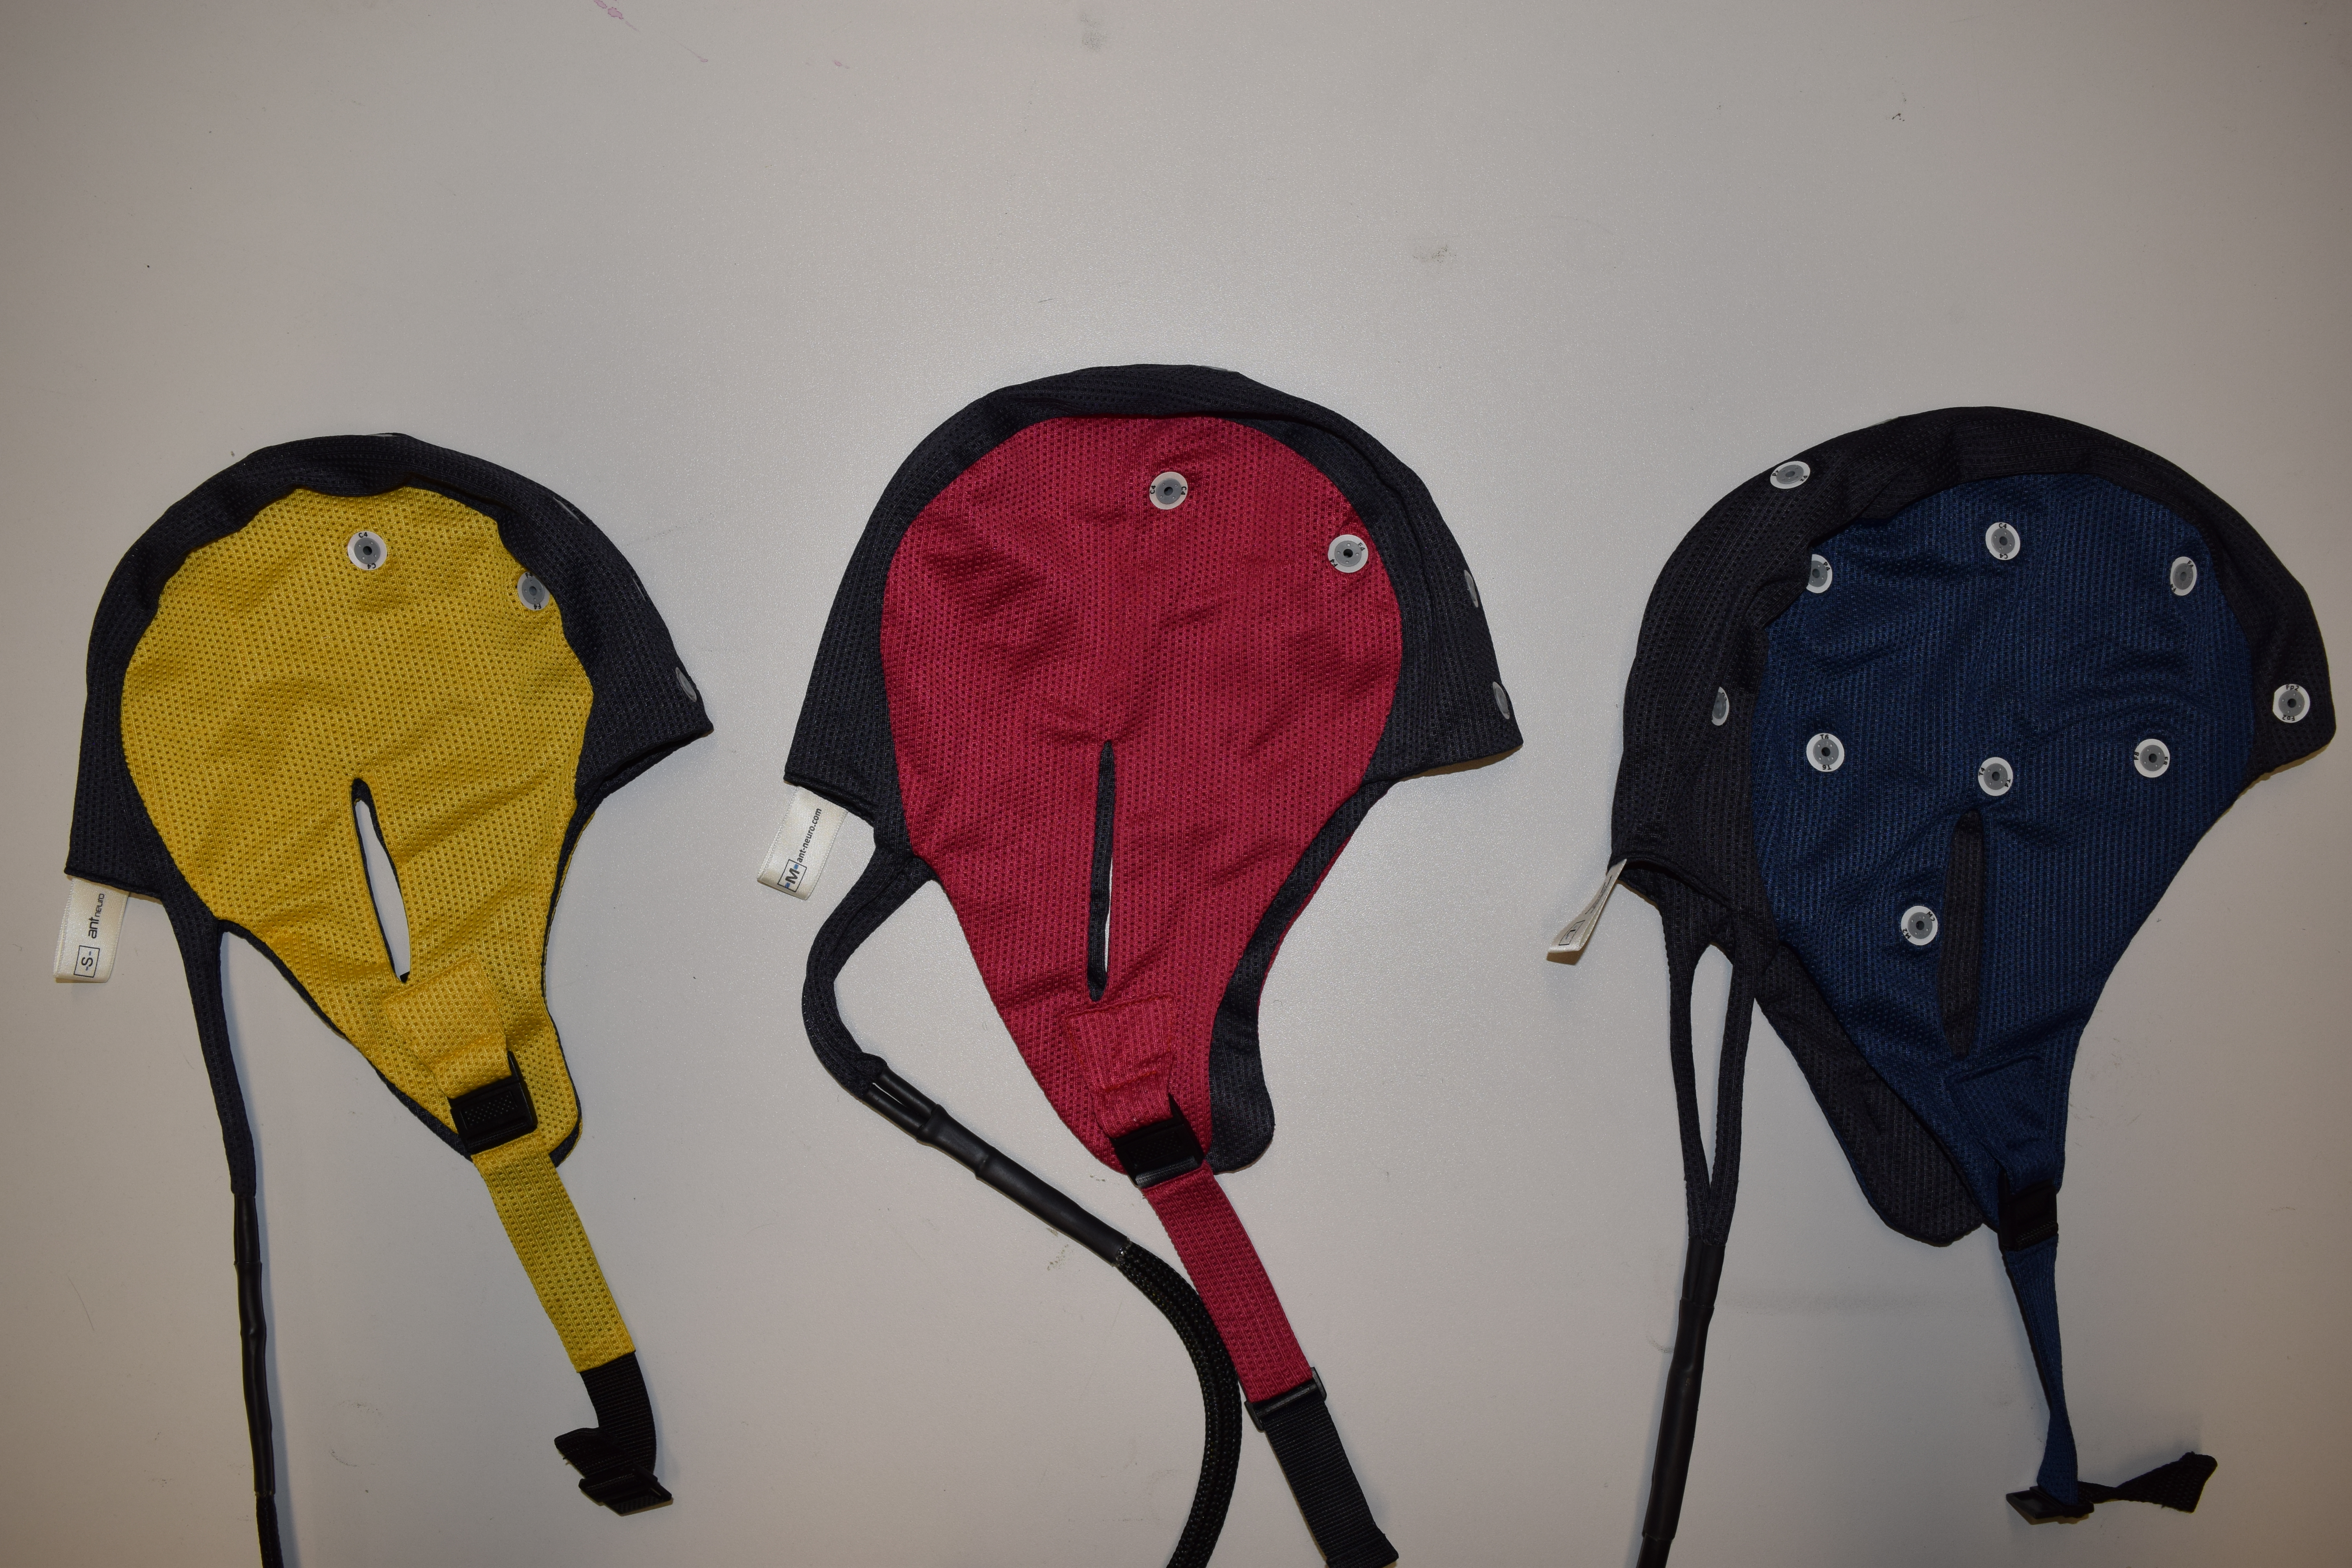
\includegraphics[width=\textwidth]{different_EEG_caps.jpg}	
		\end{subfigure}
		\hfill
		\begin{subfigure}{0.4\textwidth}
			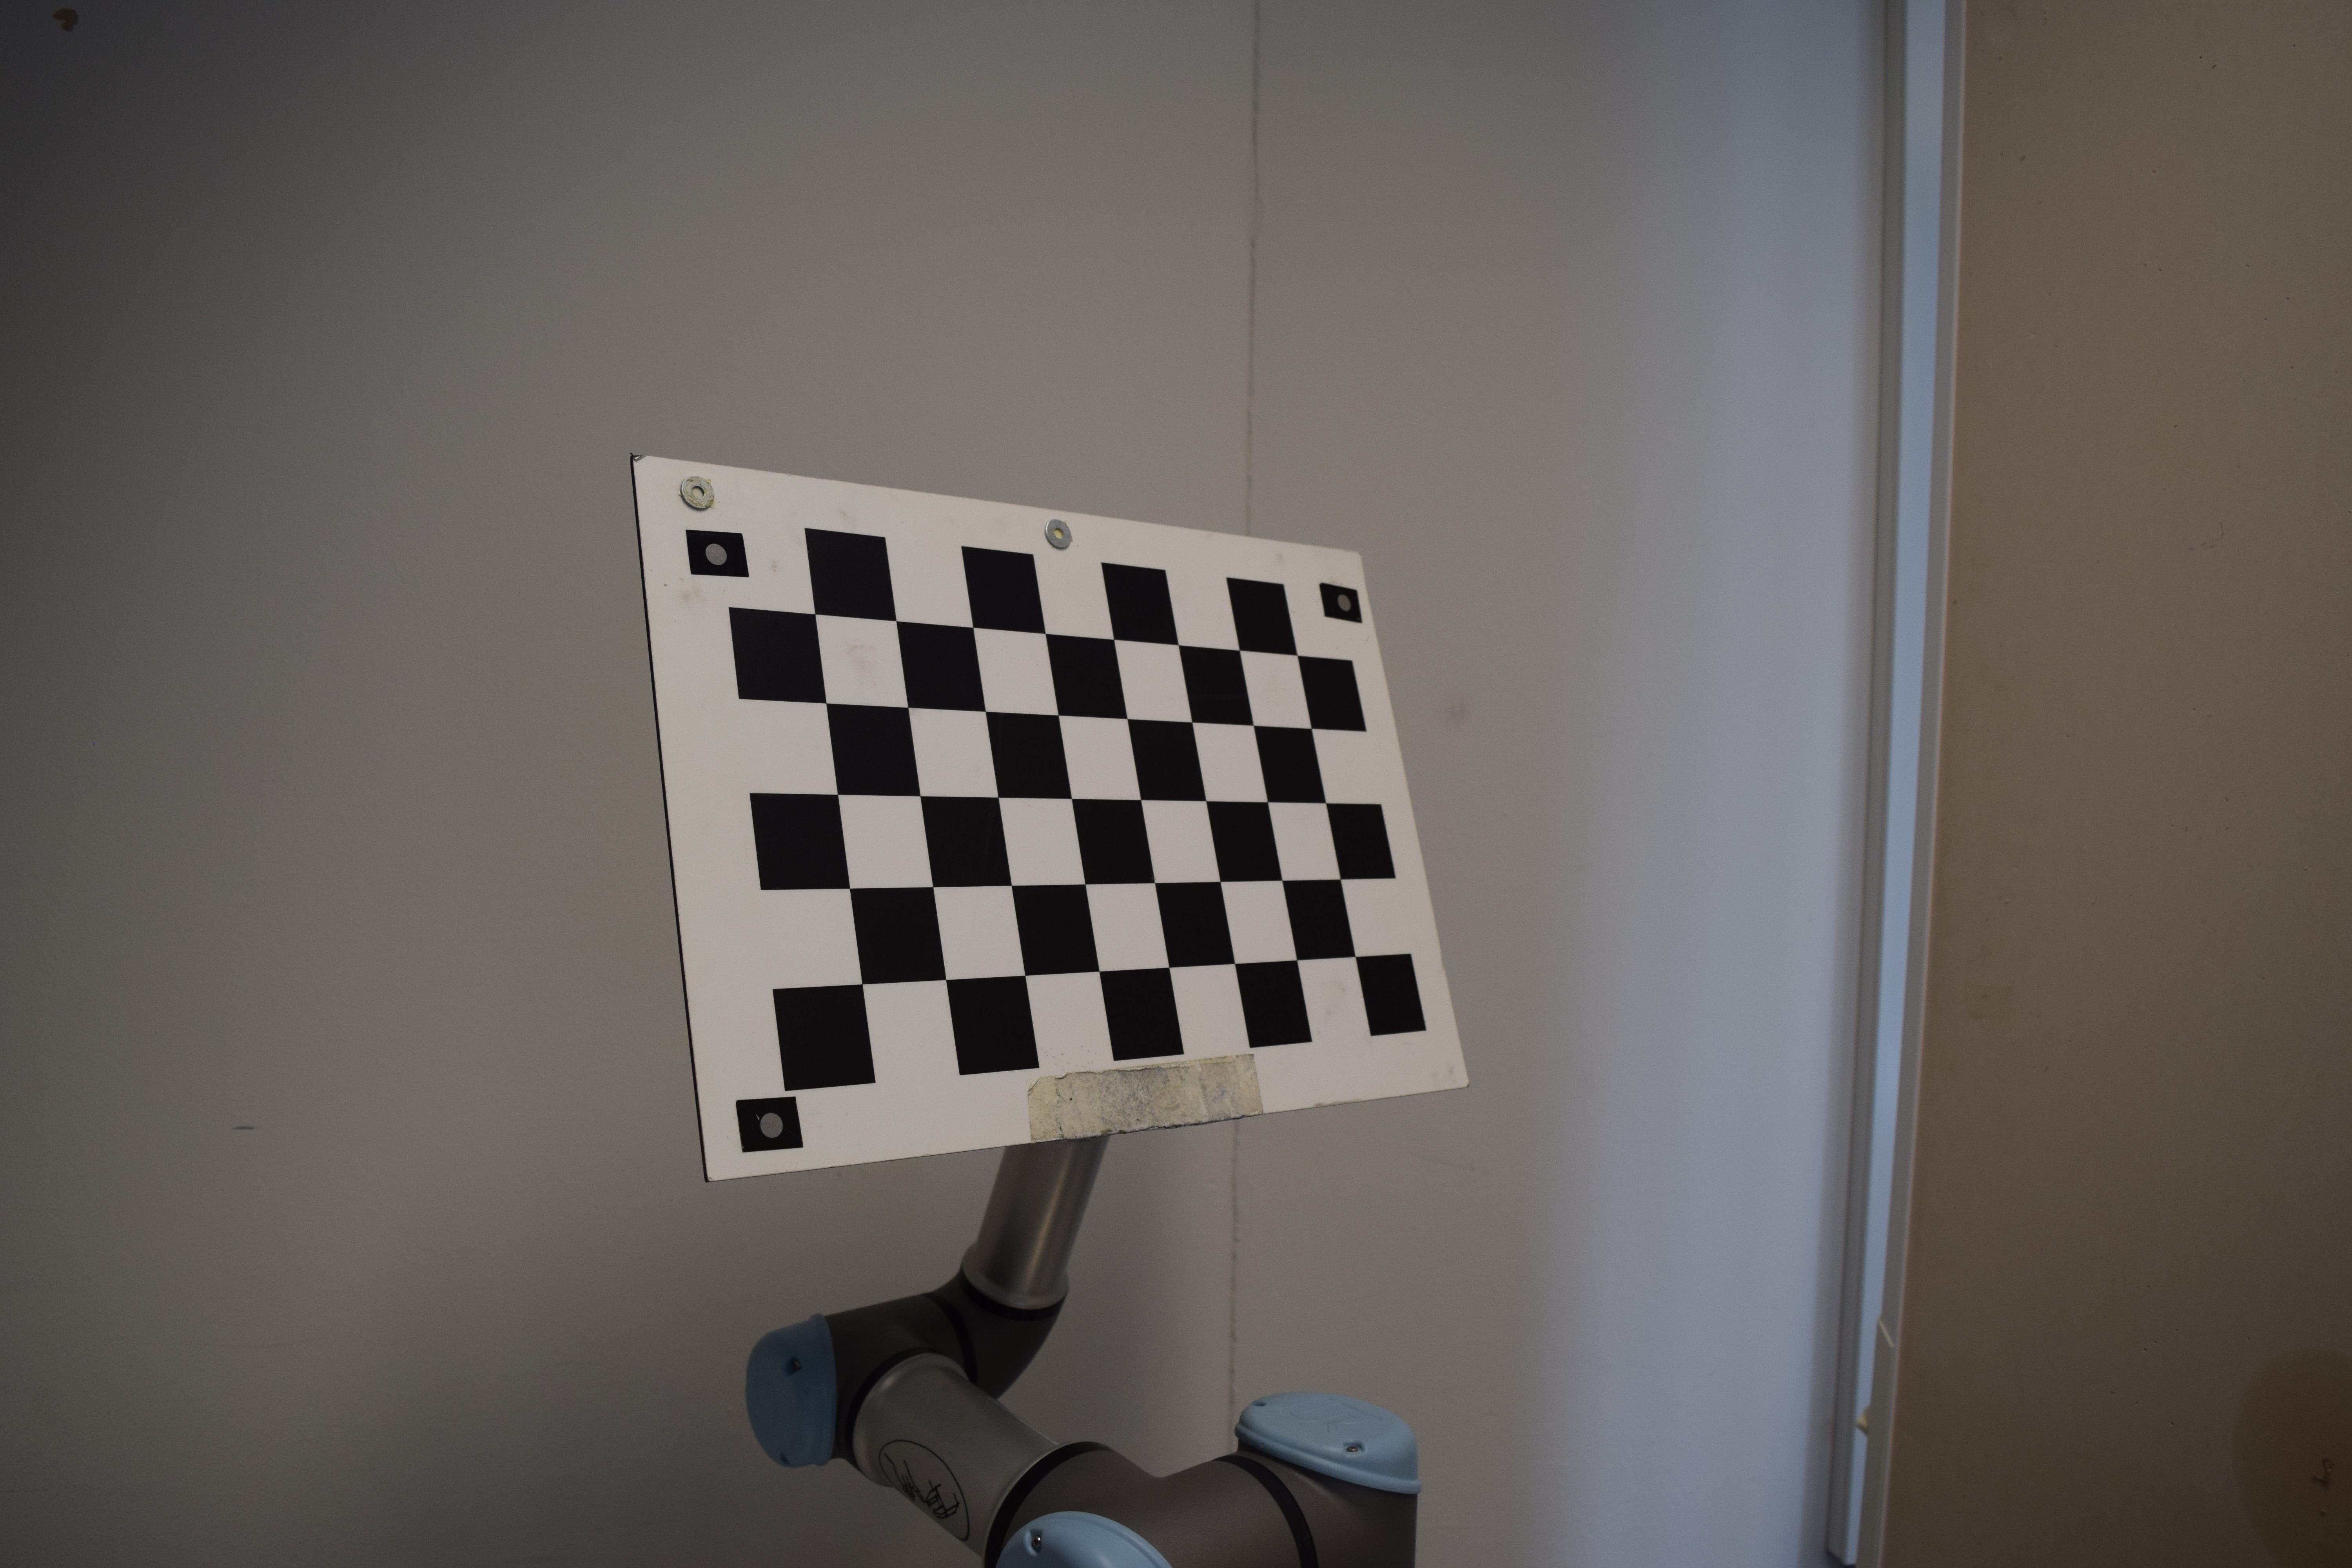
\includegraphics[width=\textwidth]{chessboard.jpg}	
		\end{subfigure}
		\begin{subfigure}{0.4\textwidth}
			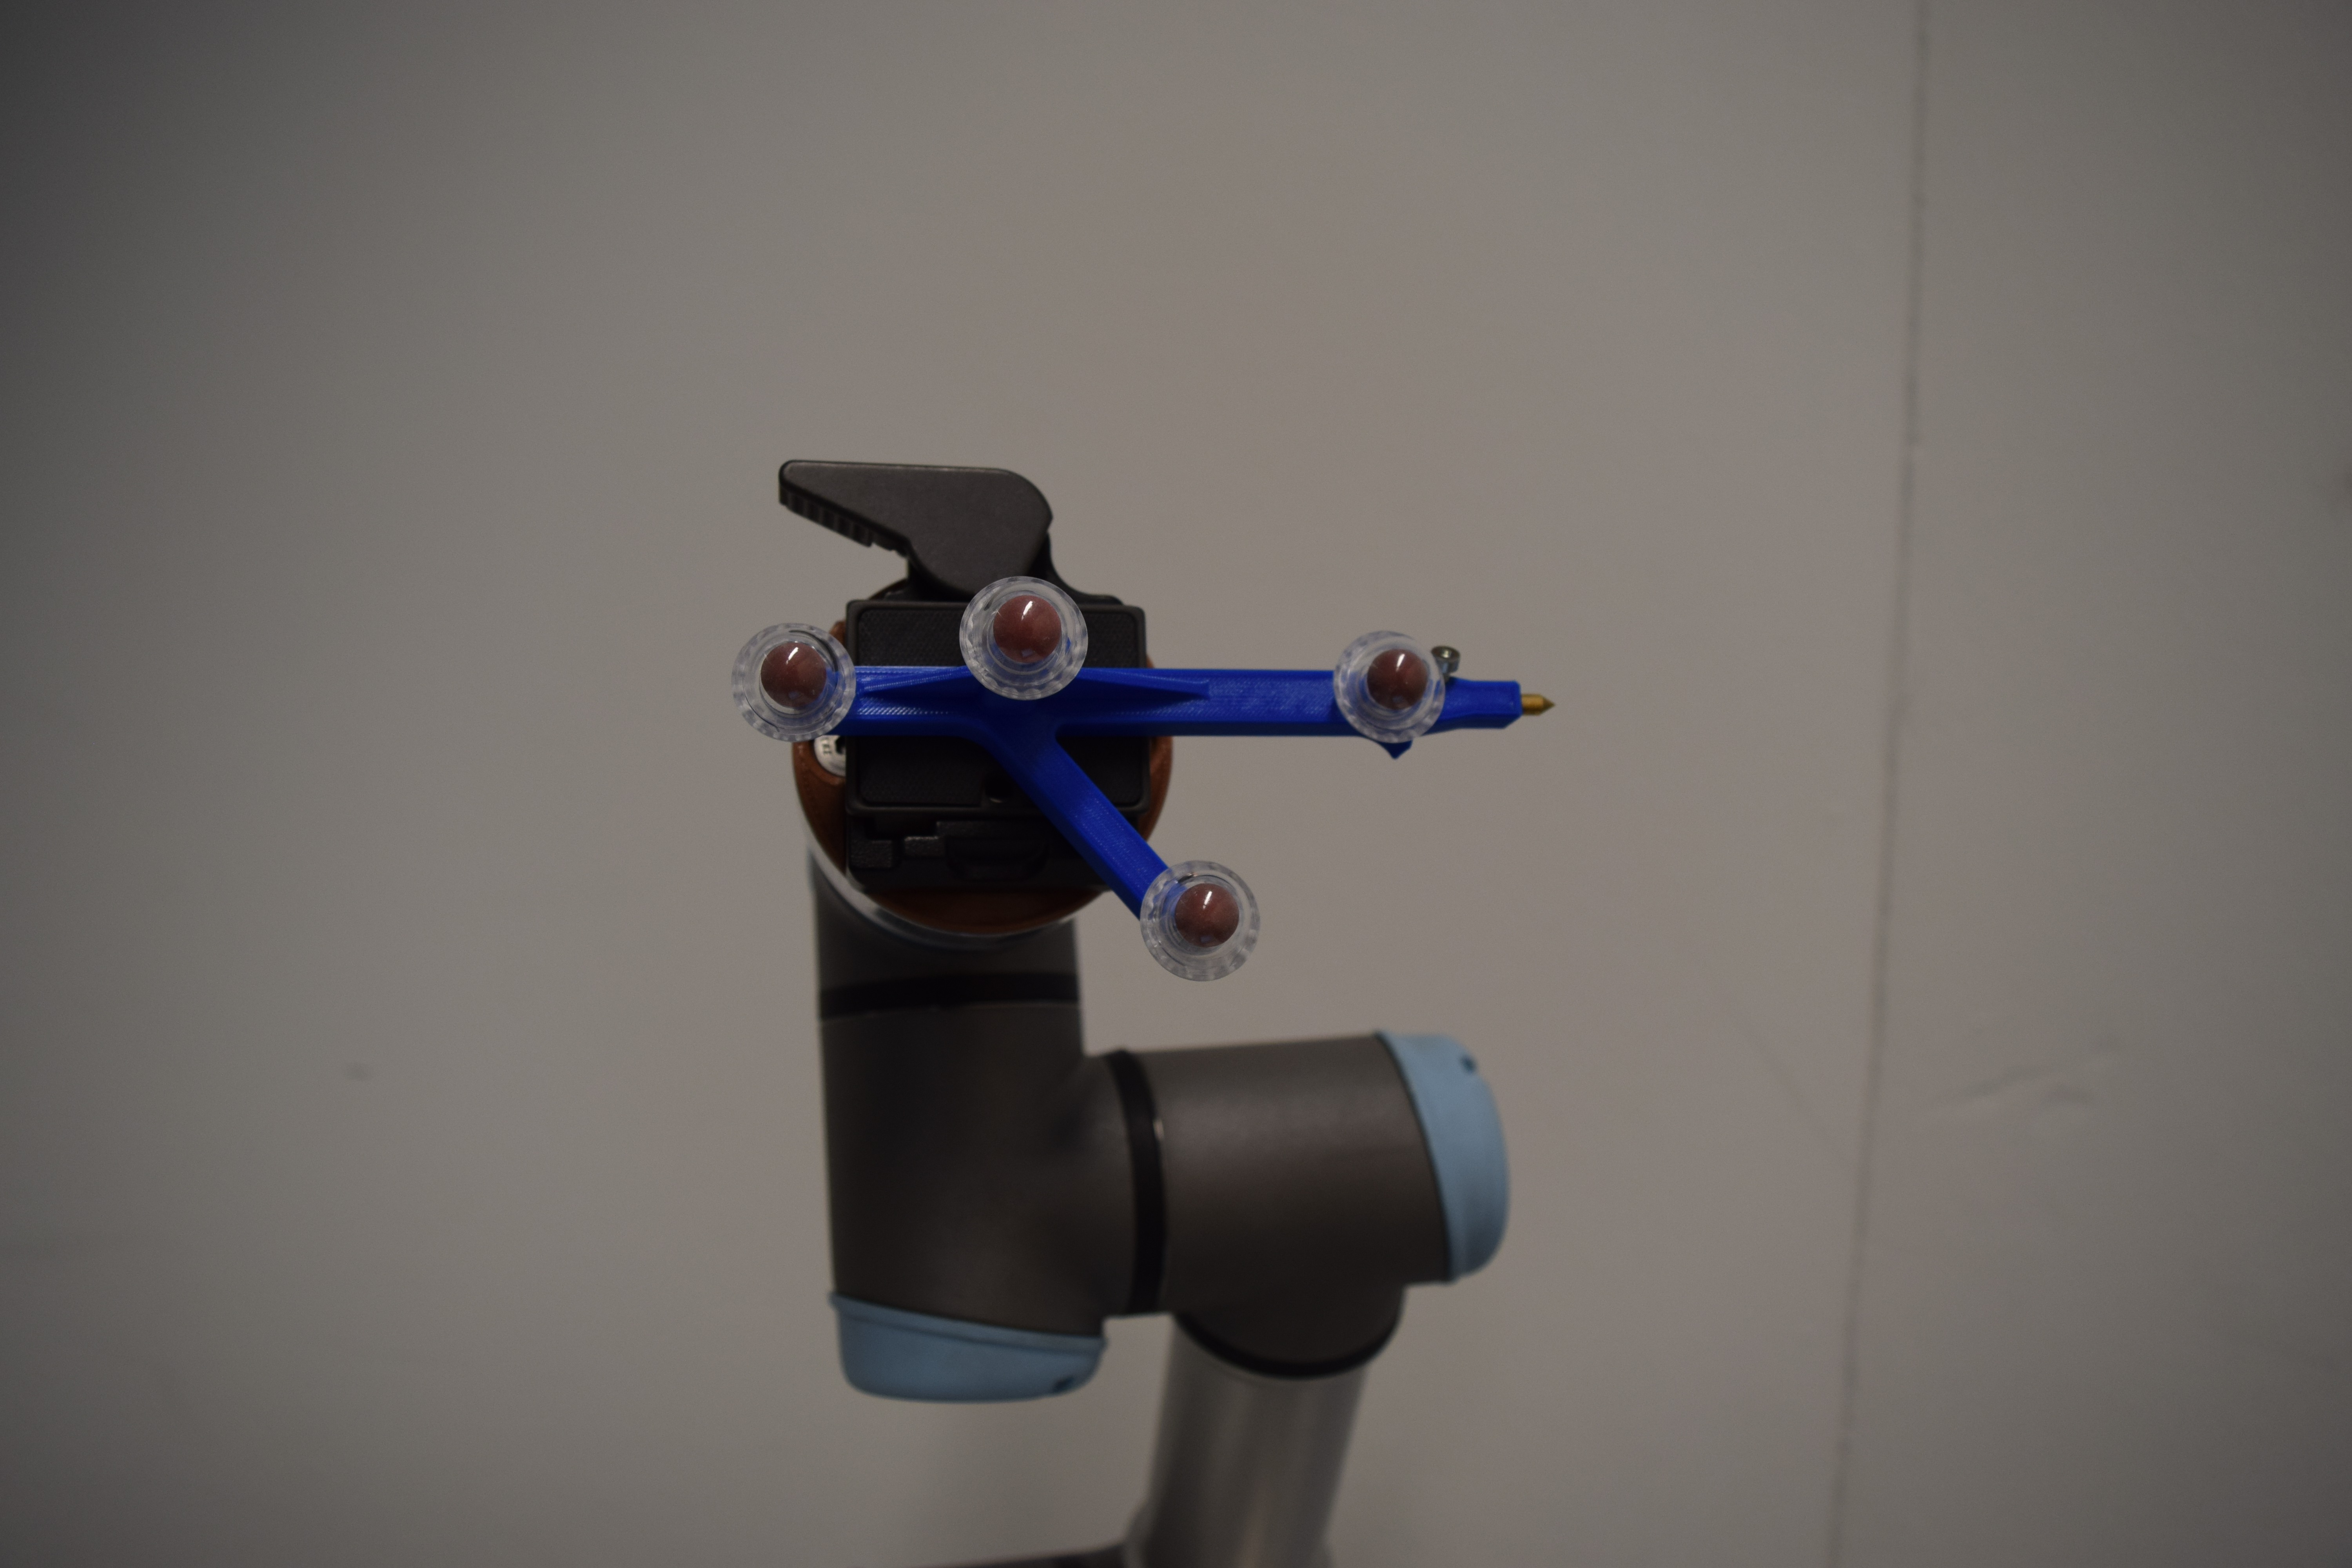
\includegraphics[width=\textwidth]{active_marker.jpg}	
		\end{subfigure}
		
		\caption{Setup consists of Microsoft kinect, Atracsys fusionTrac 500, UR3 robot, EEG caps by eemagine Medical Imaging Solutions GmbH, Berlin, and Markers.} 
		\label{fig:Eexperimental_setup}
	\end{figure}
	
\end{frame}



 
